%%% TEMPLATE-INFO
%% VERSION		: 0.11

\RequirePackage{fix-cm,cmap}

\documentclass[
    fontsize=11pt,
    paper=a4,
    abstract=true,
    numbers=noenddot,
    listof=totoc,
    bibliography=totoc,
    oneside,
    open=right,
    cleardoublepage=plain,
    parskip=half+,
    BCOR=0cm,
]{scrreprt}

\usepackage[a4paper, margin=2.5cm]{geometry}

\setcounter{tocdepth}{3}  % Inhaltsverzeichnis bis Subsubsection
\setcounter{secnumdepth}{3} % Nummerierung bis Subsubsection

% General stuff
\usepackage[utf8]{inputenc} % CHANGE HERE IF NECESSARY
\usepackage[T1]{fontenc}
\usepackage[ngerman]{babel} % last language given is used (here: english. Alternative: ngerman)
\usepackage{lmodern}

\usepackage{tikz} % used on frontpage


% Set date here
%\day=4 \month=5 \year=2023

% Set name and title
\author{Tobias Polley}
\title{Ausarbeitung zum Thema "Mapping glycoprotein structure reveals
Flaviviridae evolutionary history"}
\date{\today}

% Bibliography
\usepackage[style=numeric,giveninits=false,natbib=true,backend=biber,maxbibnames=99,defernumbers=true,language=autobib,date=long]{biblatex}
\addbibresource{literature/literature.bib}

%%%%%% %%%%%%

% Load packages ...

% Corporate Design
\usepackage{eso-pic}
\usepackage{color}
% Comment out if the RUB fonts are installed
% Link: https://noc.rub.de/~jobsanzl/latex/rubtexfonts-0.4.tar.gz
%\usepackage{rubfonts2009}
\newcommand{\setrubfontnormal}[1]{\fontfamily{rubscala}\fontsize{#1}{1}\selectfont}
\newcommand{\setrubfontextra}[1]{\fontfamily{rubflama}\fontsize{#1}{1}\selectfont}
\definecolor{rubgreen}{cmyk}{0.5,0,1,0}
\definecolor{rubblue}{cmyk}{1,0.5,0,0.6}

% Figures
\usepackage{graphicx}

% Tables
\usepackage{booktabs}
\usepackage{marvosym}
\usepackage{multirow}

% Math stuff and units
\usepackage{amsmath, amssymb, amsfonts}

% Enable quotes by \enquote{}
\usepackage[babel,english=american, german=quotes]{csquotes}

\usepackage{fontawesome5}

\usepackage{minted}
% Listings
\setminted{
	frame=single, % single, lines, leftline, topline, bottomline, none
	fontsize=\footnotesize,
        % fontsize=\scriptsize,
	linenos=true,
	numbersep=5pt,
	breaklines=true,
	breakautoindent=true,
	breakbefore=.,
	breakafter=-,
	escapeinside=~~
}
\BeforeBeginEnvironment{minted}{\smallskip}
\AfterEndEnvironment{minted}{\smallskip}
\setmintedinline{
    fontsize=\small,
    escapeinside=~~,
    breakbefore=.,
    breakafter=-:/\,
}
\newmintinline[code]{text}{}
\newmintinline[js]{javascript}{}
\newmintinline[html]{html}{}
\newmintinline[json]{json}{}

% Format page foot and header
\usepackage{scrlayer-scrpage}
\clearscrheadings
\clearscrheadfoot
\automark[section]{chapter}
\ohead{\pagemark}
\ihead{\headmark}
\pagestyle{scrheadings}

% Hyperlinks and menu for your document
% IMPORTANT: Never ever disable hyperref package. It will help your supervisor by providing clickable references and table of contents
\usepackage[breaklinks,hyperindex,colorlinks,anchorcolor=black,citecolor=black,filecolor=black,linkcolor=black,menucolor=black,urlcolor=black,pdftex,bookmarks=true,bookmarksopen=true,bookmarksnumbered=true,]{hyperref} % pagebackref: Add page number to the references where they can be found
\addto\extrasenglish{ % Capitalize Refs, Write "Listing 1" instead of just "1"
  \def\chapterautorefname{Chapter}
  \def\sectionautorefname{Section}
  \def\subsectionautorefname{Subsection}
  \def\subsubsectionautorefname{Subsubsection}
  \def\paragraphautorefname{Paragraph}
  \def\subparagraphautorefname{Subparagraph}
  \def\listingautorefname{Listing}
}

% DO NOT LOAD ANY OF YOUR PACKAGES BEYOND THIS PACKAGE

\makeatletter
\AtBeginDocument{
 \hypersetup{
   pdftitle = {\@title},
   pdfauthor = {\@author},
   pdfsubject={\@title},
   pdfkeywords={OpenID Connect, add more}, % CHANGE HERE
 }
}

% Glossary
\usepackage[toc]{glossaries}
\glsdisablehyper % Most people do not like clickable acronyms and glossary entries.
\makeglossaries

%%%%%%%%%%%
% ACRONYM %
%%%%%%%%%%%
\newacronym{bfd}{BFD}{Big Fantastic Database}
\newacronym{colabfold}{ColabFold}{Collaborative Protein Folding}
\newacronym{esmfold}{ESMFold}{Evolutionary Scale Modeling for Protein Folding}
\newacronym{evoformer}{Evoformer}{Evolutionary Transformer Module}
\newacronym{foldseek}{Foldseek}{Fast Protein Structure Search Tool}
\newacronym{gtrig}{GTR+I+G}{General Time Reversible Model with Invariant Sites and Gamma Distribution}
\newacronym{ictv}{ICTV}{International Committee on Taxonomy of Viruses}
\newacronym{iqtree}{IQ-TREE}{Efficient and Effective Phylogenetic Software Tool}
\newacronym{lgf}{LGF}{Large Genome Flaviviruses}
\newacronym{mafft}{MAFFT}{Multiple Alignment using Fast Fourier Transform}
\newacronym{msa}{MSA}{Multiple Sequence Alignment}
\newacronym{nlp}{NLP}{Natural Language Processing}
\newacronym{nsfive}{NS5}{Nichtstrukturelles Protein 5}
\newacronym{pdb}{PDB}{Protein Data Bank}
\newacronym{plddt}{pLDDT}{Predicted Local Distance Difference Test}
\newacronym{rdrp}{RdRp}{RNA-abhängige RNA-Polymerase}
\newacronym{rmsd}{RMSD}{Root-Mean-Square Deviation}
\newacronym{uniref}{UniRef90}{UniProt}

%%%%%%%%%%%
% GLOSSAR %
%%%%%%%%%%%

%% here your document starts
\begin{document}

%% switch to roman paginating for the acknowledgements, table of contents etc.
\pagenumbering{roman} % uncomment this if you like it

%% title page --- made out of expressions defined above
% Hintergrund-Makro
\newcommand\BackgroundPic{
\put(0,0){
\parbox[b][\paperheight]{\paperwidth}{%
\vfill
\centering
\includegraphics[width=\paperwidth,height=\paperheight]{images/front.png}%
\vfill
}}}

\AddToShipoutPicture*{\BackgroundPic}
\begin{titlepage}
\makeatletter

\enlargethispage{3cm}

\newgeometry{top=3cm, bottom=3cm, left=3cm, right=3cm}

\vspace*{10cm}
\begin{minipage}[b]{1\linewidth}
	\sffamily
	\hspace{-17.2mm}\includegraphics[scale=1.0]{images/rub_slogan}\\

	\textbf{\LARGE {\@title}}\\

	\Large{\@author}\\

% 	\vspace*{35mm}
	\vspace{4cm}
	\normalsize{
	Wissenschaftliche Arbeit\@~~--~~\@date\\
	Lehrstuhl der Bioinformatik\\}
	\newline
	\normalsize{
	\begin{tabular}{@{}ll@{}}
	Supervisor: & Prof. Dr. Axel Mosig \\
	Advisor: & Prof. Dr. Martin Eisenacher\\
	\end{tabular}
	}
\end{minipage}


\makeatother
\end{titlepage}
\ClearShipoutPicture


\section*{Eidesstattliche Erklärung}
{\selectlanguage{ngerman}
Ich erkläre, dass ich keine Arbeit in gleicher oder ähnlicher Fassung bereits für eine andere Prüfung an der Ruhr-Universität Bochum oder einer anderen Hochschule eingereicht habe.

\noindent
Ich versichere, dass ich diese Arbeit selbstständig verfasst und keine anderen als die angegebenen Quellen benutzt habe. Die Stellen, die anderen Quellen dem Wortlaut oder dem Sinn nach entnommen sind, habe ich unter Angabe der Quellen kenntlich gemacht.
Dies gilt sinngemäß auch für verwendete Zeichnungen, Skizzen, bildliche Darstellungen und dergleichen.

\noindent
Ich versichere auch, dass die von mir eingereichte schriftliche Version mit der digitalen Version übereinstimmt.
Ich erkläre mich damit einverstanden, dass die digitale Version dieser Arbeit zwecks Plagiatsprüfung verwendet wird.\@}

\makeatletter
\vspace{2cm}
\rule{4cm}{0.1pt} \hfill \rule{7cm}{0.1pt} \\
\hspace*{1.5cm} \textsc{Date} \hspace*{7cm} \textsc{\@author}
\makeatother

\cleardoublepage

\pagestyle{scrheadings} % reenable headers and footers

%% generate table of contents
\tableofcontents

\cleardoublepage

\pagenumbering{arabic} %switches to arabic numbers for the rest of the text
\setcounter{page}{1}

%%
%% include all your chapters as .tex files,
%% each file contains sections \section{name of section},
%% subsections \subsections{...} and so on...
%%

\chapter{Einleitung} \label{chap:einleitung}

\section{Vorstellung der Flaviviridae-Virusfamilie}
\label{sec:vorstellung-der-flaviviridae-virusfamilie}

Die Flaviviridae stellen eine der größten und vielfältigsten Familien von human- und tierpathogenen RNA-Viren dar \autocite{Simmonds2017}. Zu den wichtigsten klinischen Vertretern gehören Erreger wie das Dengue-Virus, Gelbfieber-Virus, Zika-Virus und das Hepatitis-C-Virus \autocite{Mackenzie2004}. Diese Virenfamilie unterteilt sich in die vier etablierten Gattungen: \textit{Flavivirus}, \textit{Pestivirus}, \textit{Pegivirus} und \textit{Hepacivirus} \autocite{Simmonds2017}. Die jüngere Entdeckung von Jingmenviren und sogenannten Large Genome Flaviviruses (LGFs) hat die evolutionäre Vielfalt der Flaviviridae zusätzlich erweitert und verdeutlicht deren dynamische Anpassungsfähigkeit \autocite{shiDivergentVirusesDiscovered2015}. Die Identifikation von flavivirid Sequenzen in marinen Wirbellosen und basalen Wirbeltierlinien deutet darauf hin, dass die Evolution der Flaviviridae möglicherweise der Evolution der Metazoa durch Virus-Wirt-Kodivergenz über einen Zeitraum von Hunderten von Millionen Jahren folgt.

Glycoproteine spielen innerhalb der Flaviviridae eine Schlüsselrolle, da sie entscheidend den Eintritt des Virus in Zielzellen vermitteln und somit Wirtsspezifität und Pathogenität beeinflussen \autocite{Mukhopadhyay2005}.

\begin{figure}[H]
    \centering
    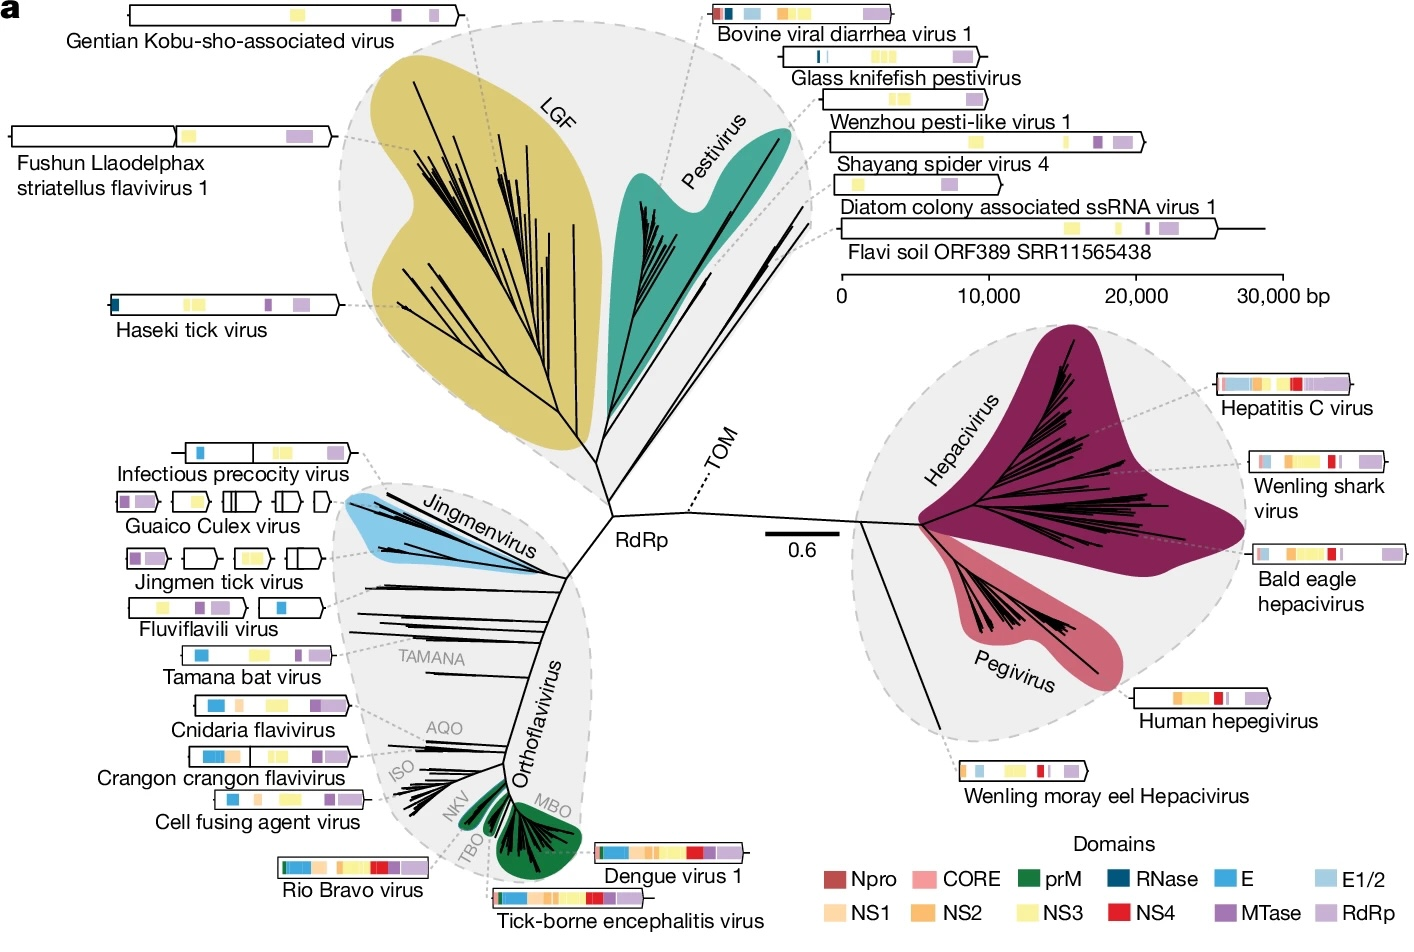
\includegraphics[width=.9\textwidth]{/workspaces/seminar-bioinformatik/images/figure1.jpeg}
    \caption{Protein Foldome der Flaviviridae-Familie.}
    \label{fig:figure1-orginal}
\end{figure}

Die Grafik zeigt die Vielfalt der Flaviviridae-Gattungen, darunter das Orthoflavivirus, Jingmenvirus, LGF und Pestivirus-ähnliche Viren. Die Fusion-Loop-Region ist ein struktureller Bestandteil, der eine zentrale Rolle bei der Membranfusion während des Viruseintritts in die Wirtszelle spielt. Die abgebildeten Schleifen sind farblich kodiert, um die unterschiedlichen Gattungen zu repräsentieren und die strukturellen Gemeinsamkeiten sowie Unterschiede hervorzuheben. Diese Analyse ist essenziell für das Verständnis der evolutionären Beziehungen und funktionellen Diversifikation innerhalb der Flaviviridae-Familie. \autocite{mifsudMappingGlycoproteinStructure2024}

\section{Bedeutung der Glycoprotein-Struktur für Evolution und Pathogenese}
\label{sec:bedeutung-der-glycoprotein-struktur-fuer-evolution-und-pathogenese}

Die Glycoproteine der Flaviviridae erfüllen zentrale Funktionen in der Virusbiologie, insbesondere durch ihre Rolle bei der Membranfusion und der Interaktion mit dem Wirtsimmunsystem \autocite{Heinz2012}. Während das E-Glycoprotein der \textit{Flavivirus}-Gattungen als prototypisches Klasse-II-Fusionsprotein gut charakterisiert ist \autocite{kuhnStructureDengueVirus2002}, weisen die Glycoproteine der Hepaciviren und Pegiviren, insbesondere die E1/E2-Komplexe, einzigartige strukturelle Eigenschaften auf. Diese könnten auf alternative Mechanismen der Membranfusion hindeuten und eine besondere evolutionäre Anpassung darstellen \autocite{Lavie2017}.

Mutationen, Rekombinationen und horizontaler Gentransfer haben entscheidend zur Diversifikation der Glycoprotein-Strukturen beigetragen und somit die Anpassungsfähigkeit der Flaviviridae an unterschiedliche ökologische Nischen gefördert \autocite{Weaver2009}. Die Untersuchung dieser strukturellen Merkmale bietet daher wertvolle Einblicke in die evolutionären Mechanismen, die zur Spezialisierung und Pathogenität der Viren führen. Besonders konservierte Regionen wie die hydrophobe Fusion-Loop-Region und transmembrane Domänen spielen eine zentrale Rolle in der Funktion der Glycoproteine und unterliegen vermutlich starkem Selektionsdruck \autocite{Modis2004}.

\section{Zielsetzung und Vorgehensweise}
\label{sec:zielsetzung-und-vorgehensweise}

Das Ziel dieser Arbeit besteht darin, die evolutionäre Geschichte und die strukturellen Eigenschaften der Glycoproteine der Flaviviridae systematisch zu untersuchen. Aufbauend auf der Arbeit von \textit{Mifsud et al.} \autocite{mifsudMappingGlycoproteinStructure2024} werden bioinformatische Methoden eingesetzt, um die Phylogenie, Proteinstrukturvorhersage und strukturelle Homologien dieser Schlüsselproteine zu analysieren. Hierbei stehen drei zentrale Fragestellungen im Fokus:

Erstens sollen die strukturellen Gemeinsamkeiten und Unterschiede der Glycoproteine zwischen den Gattungen herausgearbeitet werden. Zweitens wird untersucht, welche evolutionären Mechanismen zur Diversifikation dieser Glycoproteine beigetragen haben. Drittens sollen die funktionellen Hinweise, die sich aus konservierten und variablen Strukturmotiven ableiten lassen, analysiert werden.

Die Arbeit gliedert sich wie folgt: Kapitel~\ref{chap:methoden} beschreibt die eingesetzten bioinformatischen Verfahren zur Erstellung von Phylogenien, zur Proteinstrukturvorhersage und zur Homologiesuche. In Kapitel~\ref{chap:ergebnisse} werden die Ergebnisse zu den phylogenetischen Beziehungen und Proteinstrukturen vorgestellt. Kapitel~\ref{chap:diskussion} interpretiert diese Ergebnisse hinsichtlich ihrer evolutionären und funktionellen Bedeutung sowie methodischer Limitationen. Abschließend fasst Kapitel~\ref{chap:schlussfolgerung} die zentralen Erkenntnisse zusammen und gibt einen Ausblick auf zukünftige Forschungsansätze.

\chapter{Methoden} \label{chap:methoden}

\section{Phylogenetische Analyse} \label{sec:phylogenetische-analyse}

Für die phylogenetische Untersuchung der Flaviviridae-Familie wurden 458 vollständige Genomsequenzen aus öffentlichen Datenbanken wie GenBank extrahiert und sorgfältig kuratiert, um eine hohe Datenqualität sicherzustellen \autocite{mifsudMappingGlycoproteinStructure2024}. Als phylogenetischer Marker diente das \gls{nsfive}-Gen, welches für die RNA-abhängige RNA-Polymerase (\gls{rdrp}) kodiert und aufgrund seiner hohen Konservierung innerhalb der Flaviviridae ideal für phylogenetische Analysen ist \autocite{Koonin1991}.

Die Sequenzen wurden mit dem Programm \gls{mafft} zu einem Multiplen Sequenzalignment (\gls{msa}) ausgerichtet \autocite{Katoh2013}. \gls{mafft} ermöglicht durch effiziente Algorithmen und die Nutzung von Fourier-Transformationen eine genaue Ausrichtung großer Datensätze, wodurch konservierte und variable Regionen innerhalb der Sequenzen identifiziert werden können. Die detaillierten mathematischen Methoden zur Erstellung der \glspl{msa} sind im Anhang \ref{chap:mathematische-formeln} beschrieben.

Anschließend wurde das \gls{msa} verwendet, um einen phylogenetischen Baum zu rekonstruieren. Hierfür kam die Maximum-Likelihood-Methode zum Einsatz, implementiert im Programm \gls{iqtree} \autocite{Nguyen2015}. Das \gls{gtrig}-Substitutionsmodell wurde gewählt, da es eine flexible Modellierung von Nukleotidsubstitutionen ermöglicht und für komplexe phylogenetische Analysen geeignet ist \autocite{Tavare1986}. Die mathematischen Grundlagen der Maximum-Likelihood-Methode und des verwendeten Substitutionsmodells sind im Anhang \ref{chap:mathematische-formeln} dargestellt.

Die Robustheit der phylogenetischen Baumtopologie wurde durch Bootstrapping mit 1.000 Wiederholungen getestet \autocite{Felsenstein1985}. Dieses statistische Verfahren prüft die Zuverlässigkeit der Knoten im Baum, indem es wiederholt Stichproben aus den Daten zieht und die Baumrekonstruktion durchführt. Hohe Bootstrap-Werte (in der Regel über 70\text{\%}) deuten auf eine starke Unterstützung der entsprechenden Knoten hin.

Durch diese methodische Vorgehensweise konnten die phylogenetischen Beziehungen innerhalb der Flaviviridae-Familie detailliert untersucht und Hauptkladen identifiziert werden, die mit den beobachteten Unterschieden in den Glycoprotein-Strukturen korrelieren.

\section{Proteinstrukturvorhersage: ColabFold und ESMFold Methoden} \label{sec:colabfold-esmfold}

Für die Vorhersage der dreidimensionalen Strukturen der Glycoproteine der Flaviviridae wurden zwei fortschrittliche bioinformatische Methoden eingesetzt: \gls{colabfold} und \gls{esmfold}. Beide basieren auf tiefen neuronalen Netzwerken, nutzen jedoch unterschiedliche Ansätze zur Proteinstrukturvorhersage und ergänzen sich somit in ihrer Anwendung.

\gls{colabfold} ist eine optimierte und zugängliche Implementierung von AlphaFold2, die es ermöglicht, Proteinstrukturvorhersagen effizient und ressourcenschonend durchzuführen \autocite{Mirdita2022}. AlphaFold2 hat das Feld der Proteinstrukturvorhersage revolutioniert, indem es tiefe neuronale Netzwerke mit evolutionären Informationen aus \glspl{msa} kombiniert, um hochpräzise Strukturvorhersagen zu generieren \autocite{Jumper2021}.

Der Vorhersageprozess mit \gls{colabfold} umfasst mehrere Schritte. Zunächst wird für jede Glycoprotein-Sequenz ein \gls{msa} erstellt, indem homologe Sequenzen aus großen Datenbanken wie \gls{uniref}, MGnify und der \gls{bfd} identifiziert werden. Dieses \gls{msa} dient dazu, evolutionäre Informationen zu extrahieren, indem es konservierte Positionen und ko-evolutionäre Signale zwischen Aminosäuren erkennt. Anschließend werden die Sequenz und das \gls{msa} in das AlphaFold2-Modell eingegeben. Das Modell besteht aus einem \gls{evoformer}-Modul, das Transformer-Architekturen verwendet, um Sequenzinformationen und \gls{msa}-Daten zu verarbeiten und langreichweitige Wechselwirkungen zwischen Aminosäuren zu modellieren. Schließlich sagt ein Strukturvorhersagekopf die dreidimensionalen Koordinaten der Proteinatome voraus, wobei sowohl geometrische als auch physikalische Constraints berücksichtigt werden. Die Qualität der Vorhersagen wird durch den \gls{plddt} bewertet, der einen Vertrauenswert für jede Position im Protein liefert.

Im Gegensatz dazu verwendet \gls{esmfold} einen proteinsprachbasierten Ansatz, der direkt aus Einzelsequenzen lernt, ohne auf \glspl{msa} angewiesen zu sein \autocite{linEvolutionaryscalePredictionAtomiclevel2023}. \gls{esmfold} basiert auf dem ESM-2-Modell, einem großen Transformer-Sprachmodell, das auf Millionen von Proteinsequenzen trainiert wurde. Es nutzt Techniken aus der natürlichen Sprachverarbeitung (\gls{nlp}), um Muster und Regularitäten in Proteinsequenzen zu erkennen. Die Proteinsequenz wird in das Modell eingegeben, das eine kontextabhängige Repräsentation jeder Aminosäure erzeugt. Diese Repräsentationen werden dann verwendet, um die dreidimensionalen Koordinaten der Proteinstruktur vorherzusagen, indem Abstände und Orientierungen zwischen Aminosäuren geschätzt werden. Obwohl \gls{esmfold} keine \glspl{msa} verwendet, kann es dennoch genaue Vorhersagen liefern, insbesondere bei Proteinen mit wenigen oder keinen homologen Sequenzen.

Beide Methoden wurden angewandt, um die Strukturen der Glycoproteine der verschiedenen Flaviviridae-Gattungen vorherzusagen. Durch den Einsatz von \gls{colabfold} konnten wir von den evolutionären Informationen profitieren, die in den \glspl{msa} enthalten sind, was insbesondere bei konservierten Proteinen zu präzisen Vorhersagen führt. \gls{esmfold} ergänzte diese Vorhersagen, indem es auch für hochdivergente Sequenzen zuverlässige Ergebnisse lieferte, bei denen wenige homologe Sequenzen verfügbar sind.

Die vorhergesagten Strukturen wurden anschließend validiert und verglichen. Eine Strukturüberlagerung der Modelle aus \gls{colabfold} und \gls{esmfold} ermöglichte die Beurteilung der räumlichen Übereinstimmung, und die Berechnung der Root-Mean-Square Deviation (\gls{rmsd}) lieferte quantitative Maße für Unterschiede zwischen den Strukturen. Die \gls{plddt}-Werte wurden analysiert, um Bereiche hoher und niedriger Vorhersagegenauigkeit zu identifizieren. Besondere Aufmerksamkeit wurde konservierten strukturellen Motiven wie den hydrophoben Fusion-Loops geschenkt, die für die Funktion der Glycoproteine essenziell sind \autocite{Modis2004}.

Die Vorhersagen der Glycoprotein-Strukturen ermöglichten es, funktionelle Domänen zu identifizieren und Unterschiede zwischen den Gattungen der Flaviviridae zu analysieren. So konnten wir beispielsweise Variationen in den Oberflächenexpositionen potenzieller Rezeptorbindungsstellen feststellen, was auf unterschiedliche Mechanismen des Viruseintritts und der Wirtsspezifität hindeutet \autocite{Lavie2017}.

Es ist jedoch zu beachten, dass die Genauigkeit der Vorhersagen von mehreren Faktoren abhängt. Bei Proteinen mit hoher Sequenzdivergenz oder wenigen verfügbaren homologen Sequenzen kann die Vorhersagegenauigkeit beeinträchtigt sein. Während \gls{colabfold} auf die Verfügbarkeit umfangreicher Sequenzdaten angewiesen ist, zeigt \gls{esmfold} Vorteile bei der Vorhersage von Proteinen mit geringer Homologie zu bekannten Strukturen. Dennoch ist die Interpretation der Vertrauenswerte und Vorhersagen im Kontext biologischer Funktion und experimenteller Validierung essenziell.

Die Kombination von \gls{colabfold} und \gls{esmfold} ermöglichte es, ein umfassendes Bild der Glycoprotein-Strukturen der Flaviviridae zu erhalten. Diese Strukturen bilden die Grundlage für weiterführende Studien zur Funktion, Evolution und potenziellen therapeutischen Zielstrukturen innerhalb dieser bedeutenden Virusfamilie.

\section{Homologiesuche: Anwendung von Foldseek} \label{sec:foldseek}

Zur Untersuchung der evolutionären Beziehungen zwischen den Glycoproteinen der Flaviviridae und zur Identifizierung struktureller Homologien wurde das Programm \gls{foldseek} eingesetzt \autocite{vankempenFastAccurateProtein2024}. \gls{foldseek} ermöglicht einen schnellen und effizienten Vergleich von Proteinstrukturen auf Basis geometrischer und physikochemischer Eigenschaften, was besonders für große Datensätze und hochdivergente Sequenzen geeignet ist.

Die vorhergesagten Glycoprotein-Strukturen aus \gls{colabfold} und \gls{esmfold} wurden mit \gls{foldseek} gegen die \gls{pdb} durchsucht, um potenzielle strukturelle Homologien zu bekannten Proteinen zu identifizieren. Dabei werden die dreidimensionalen Koordinaten der Proteine in vereinfachte Merkmalsrepräsentationen umgewandelt, die charakteristische strukturelle Merkmale erfassen \autocite{vankempenFastAccurateProtein2024}. Durch effiziente Algorithmen können so strukturelle Ähnlichkeiten auch bei geringer Sequenzidentität erkannt werden, was traditionelle sequenzbasierte Methoden wie BLAST nicht leisten \autocite{Altschul1990}.

Die Ergebnisse wurden anhand von Alignment-Scores und \gls{rmsd}-Werten bewertet, um die Qualität der Übereinstimmungen zu quantifizieren. Hohe Übereinstimmungen deuteten auf konservierte Faltungsmuster hin, insbesondere die Klasse-II-Fusionsproteinfaltung, die für die Funktion der Glycoproteine essenziell ist \autocite{Kielian2006}. Trotz hoher Sequenzdivergenz konnten gemeinsame strukturelle Merkmale identifiziert werden, was auf eine konservierte Funktion und einen gemeinsamen evolutionären Ursprung hindeutet \autocite{Chothia1986}.

Die Übereinstimmung zwischen zwei Strukturen wird durch die \gls{rmsd} bewertet, wobei die detaillierte mathematische Herleitung im Anhang \ref{chap:mathematische-formeln} erläutert wird.

Die Integration der \gls{foldseek}-Ergebnisse mit den phylogenetischen Analysen und den Proteinstrukturvorhersagen ermöglichte ein umfassendes Verständnis der evolutionären Beziehungen innerhalb der Flaviviridae. Diskrepanzen zwischen sequenzbasierten Phylogenien und strukturbasierten Homologien wurden analysiert, um mögliche Fälle von konvergenter Evolution oder funktioneller Anpassung zu identifizieren \autocite{Doolittle1999}.

Durch diese methodische Vorgehensweise konnten funktionelle Domänen innerhalb der Glycoproteine identifiziert und neue Erkenntnisse über ihre evolutionäre Diversität gewonnen werden. Die strukturelle Homologiesuche mit \gls{foldseek} erwies sich somit als wertvolles Werkzeug zur Erweiterung des Verständnisses der Flaviviridae-Proteinstrukturen über die Grenzen sequenzbasierter Analysen hinaus.

\chapter{Ergebnisse} \label{chap:ergebnisse}

\section{Phylogenetische Strukturen und Klassifizierung} \label{sec:phylogenetische-strukturen}

Die phylogenetische Analyse der Flaviviridae-Familie, basierend auf den \gls{nsfive}-Sequenzen von 458 vollständigen Virengenomen, führte zu einer klaren Aufteilung in drei Hauptkladen. Die Maximum-Likelihood-Methode wurde zur Rekonstruktion des phylogenetischen Baumes verwendet, wobei das Substitutionsmodell \gls{gtrig} zum Einsatz kam. Die resultierende Topologie wurde durch hohe Bootstrap-Werte ($>$90\%) unterstützt und ermöglicht eine robuste Klassifizierung \autocite{mifsudMappingGlycoproteinStructure2024}.

Die erste Hauptklade umfasst klassische Vertreter der Gattung \textit{Flavivirus}, zu denen das Dengue-Virus, Zika-Virus und Gelbfieber-Virus gehören. Diese Gruppe zeigt eine bemerkenswerte Konservierung des NS5-Gens, was auf eine enge evolutionäre Verwandtschaft hindeutet. Die Glycoprotein-Strukturen, insbesondere das E-Glycoprotein, sind stark konserviert und spielen eine zentrale Rolle beim Eintritt in Wirtszellen \autocite{Rey1995}.

In der zweiten Hauptklade wurden die Gattungen \textit{Pegivirus} und \textit{Hepacivirus} zusammengefasst. Hier zeigt sich eine größere genetische Diversität, insbesondere in den Glycoprotein-Genen. Die strukturelle Variabilität der E1/E2-Glycoproteine deutet auf spezifische Mechanismen der Wirtsspezifität und des Viruseintritts hin \autocite{Vieyres2013}.

Die dritte Hauptklade vereint die Gattungen \textit{Pestivirus}, \textit{Jingmenvirus} und die sogenannten Large Genome Flaviviruses (LGFs). Diese Gruppe weist stark divergente Sequenzen und eine hohe strukturelle Vielfalt in den Glycoproteinen auf. Auffällig sind hier Anpassungen in transmembranen Domänen und möglichen Rezeptorbindungsstellen, die auf spezifische Wirt-Interaktionen hinweisen \autocite{Tautz2015}.

\section{Glycoprotein-Divergenz: Unterschiede zwischen Gattungen} \label{sec:glycoprotein-divergenz}

Die Vorhersage der Glycoprotein-Strukturen mithilfe von \gls{colabfold} und \gls{esmfold} zeigte sowohl konservierte als auch variable Merkmale zwischen den Hauptkladen.

Bei den \textit{Flaviviren} erwies sich das E-Glycoprotein als stark konserviert, insbesondere in der hydrophoben Fusion-Loop-Region und den transmembranen Domänen. Die typische Klasse-II-Faltungsarchitektur mit drei Domänen aus $\beta$-Faltblättern wurde bestätigt und unterstreicht die essenzielle Funktion dieser Region \autocite{Modis2004}.

Im Gegensatz dazu zeigten die Glycoproteine der \textit{Hepaciviren} und \textit{Pegiviren}, die aus E1/E2-Komplexen bestehen, signifikante strukturelle Unterschiede. Vor allem die Oberflächenexpositionen potenzieller Rezeptorbindungsstellen variieren stark und könnten die breite Wirtsspezifität und unterschiedliche Pathogenitätsprofile dieser Gattungen erklären \autocite{Lavie2017}.

\begin{figure}[H]
    \centering
    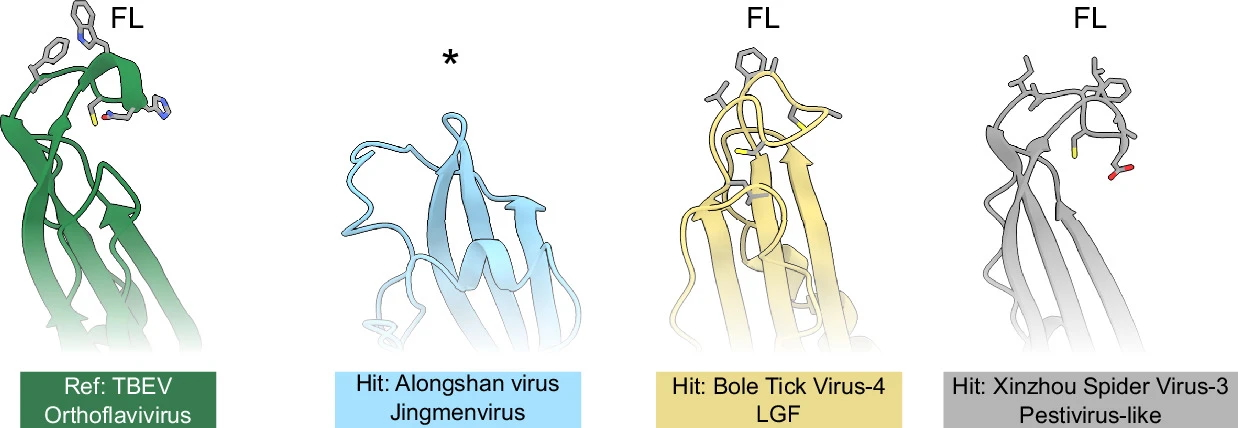
\includegraphics[width=\textwidth]{/workspaces/seminar-bioinformatik/images/figure6.jpeg}
    \caption{Strukturelle Unterschiede der Fusion-Loop-Regionen}
    \label{fig:figure6-orginal}
\end{figure}

Die größte strukturelle Diversität wurde in den Glycoproteinen der \textit{Pestiviren} und \textit{Jingmenviren} beobachtet. Unterschiede in der Anzahl und Position der transmembranen Domänen sowie Variationen in den extrazellulären Regionen deuten auf funktionelle Anpassungen hin, die spezifische Interaktionen mit Wirtsorganismen ermöglichen \autocite{Tautz2015}.

Trotz der beobachteten Variabilität wurden konservierte Motive wie die hydrophoben Fusion-Loops und transmembranen Segmente identifiziert, die für die grundlegende Funktion der Glycoproteine entscheidend sind und unter starkem Selektionsdruck stehen \autocite{Modis2004}.

\section{Spezifische Strukturmerkmale (Fusion-Loop und transmembrane Regionen)} \label{sec:spezifische-strukturmerkmale}

Die detaillierte Analyse der Fusion-Loop-Regionen und transmembranen Segmente der Glycoproteine lieferte wichtige Einblicke in deren funktionelle Rollen. Die Fusion-Loops bestehen aus konservierten hydrophoben Aminosäureresten, die essenziell für die Membranfusion sind. Bei den \textit{Flaviviren} zeigt die Fusion-Loop eine charakteristische Schleifenstruktur, die von Glycinresten flankiert wird und Flexibilität unter sauren pH-Bedingungen ermöglicht \autocite{Rey1995}. Im Gegensatz dazu deuten Unterschiede in Sequenz und Sekundärstruktur bei \textit{Hepaciviren} und \textit{Pegiviren} auf alternative Mechanismen der Membranfusion hin \autocite{Lavie2017}.

Die transmembranen Regionen variieren stark zwischen den Gattungen. Während \textit{Flaviviren} typischerweise nur eine einzelne transmembrane Domäne am C-Terminus des E-Glycoproteins besitzen, weisen \textit{Pestiviren} und \textit{Hepaciviren} mehrere transmembrane Segmente auf. Diese Variationen könnten die Organisation der Glycoproteine in der viralen Membran beeinflussen und somit die Virusassemblierung und -freisetzung modulieren \autocite{peninStructureFunctionMembrane2004}. Zusätzlich wurden Signalpeptide und Ankersequenzen identifiziert, die eine wichtige Rolle für die Lokalisierung und Stabilität der Proteine spielen \autocite{Ashkenazy2016}.

\chapter{Diskussion} \label{chap:diskussion}

\section{Evolutionäre Bedeutung der Glycoprotein-Divergenz} \label{sec:evolutionaere-bedeutung-der-glycoprotein-divergenz}

Die Ergebnisse dieser Studie unterstreichen die zentrale Rolle der Glycoproteine in der Evolution und Anpassung der Flaviviridae-Familie. Die beobachtete Diversität der Glycoprotein-Strukturen spiegelt eine komplexe evolutionäre Dynamik wider, die durch Selektionsdruck, Wirtsspezifität und ökologische Nischen geprägt ist \autocite{mifsudMappingGlycoproteinStructure2024}.

Die hohe Konservierung der hydrophoben Fusion-Loops und transmembranen Domänen über verschiedene Gattungen hinweg deutet darauf hin, dass diese Regionen essenziell für die grundlegenden Funktionen des Virus sind, insbesondere für die Membranfusion und den Eintritt in die Wirtszelle \autocite{Rey1995} \autocite{Modis2004}. Diese konservierten Strukturen stehen vermutlich unter starkem evolutionärem Selektionsdruck, da Änderungen in diesen Bereichen die Virulenz oder Infektiosität des Virus erheblich beeinträchtigen könnten.

Gleichzeitig weisen die variablen Regionen der Glycoproteine, wie beispielsweise die Oberflächenexpositionen und Glycosylierungsstellen, eine größere Diversität auf. Diese Unterschiede könnten auf adaptive Mechanismen zurückzuführen sein, die es den Viren ermöglichen, an verschiedene Wirtsorganismen anzupassen oder das Immunsystem des Wirts zu umgehen \autocite{Lavie2017}. Beispielsweise könnten Variationen in den E1/E2-Komplexen der Hepaciviren dazu beitragen, die breite Wirtsspezifität und die Fähigkeit zur chronischen Infektion zu erklären \autocite{Vieyres2013}.

Die strukturellen Unterschiede zwischen den Gattungen könnten auch das Ergebnis von Rekombinationsereignissen oder horizontalem Gentransfer sein, was zur Entstehung neuer Virusstämme mit unterschiedlichen Pathogenitätsprofilen führt \autocite{Weaver2009}. Diese Mechanismen tragen zur genetischen Vielfalt der Flaviviridae bei und ermöglichen es den Viren, sich an veränderte Umweltbedingungen oder Wirtsimmunantworten anzupassen.

Insgesamt betonen die Ergebnisse die Bedeutung der Glycoprotein-Divergenz als treibende Kraft in der Evolution der Flaviviridae und liefern wichtige Einblicke in die molekularen Mechanismen der Virusadaption und Pathogenese.

\section{Methodologische Limitierungen und Unsicherheiten} \label{sec:methodologische-limitierungen-und-unsicherheiten}

Obwohl die angewandten Methoden, insbesondere die Verwendung von ColabFold und ESMFold für die Proteinstrukturvorhersage, robuste Ergebnisse lieferten, gibt es einige methodologische Limitierungen, die berücksichtigt werden müssen.

Erstens hängt die Genauigkeit der Strukturvorhersagen von der Qualität der zugrunde liegenden Modelle und Algorithmen ab \autocite{Jumper2021}. Insbesondere bei Proteinen mit geringer Sequenzähnlichkeit zu bekannten Strukturen kann die Zuverlässigkeit der Vorhersagen abnehmen. Dies betrifft vor allem die Glycoproteine der Pestiviren und Jingmenviren, bei denen wenig experimentelle Strukturdaten verfügbar sind.

Zweitens ist die Abhängigkeit von in silico Methoden ohne experimentelle Validierung eine potenzielle Quelle für Unsicherheiten. Obwohl die Vorhersagen durch konsistente Ergebnisse zwischen ColabFold und ESMFold gestützt werden, sind experimentelle Strukturanalysen, wie zum Beispiel durch Röntgenkristallographie oder Kryo-Elektronenmikroskopie, notwendig, um die Modelle zu bestätigen \autocite{Callaway2020}.

Drittens könnten die phylogenetischen Analysen durch Faktoren wie unvollständige Sequenzdaten, Rekombinationsereignisse oder unterschiedliche Evolutionsraten beeinflusst werden \autocite{Felsenstein1985}. Die Verwendung eines einzelnen phylogenetischen Markers (NS5-Gen) könnte die Auflösung der phylogenetischen Beziehungen einschränken. Eine multimarkergestützte Analyse könnte hier zu detaillierteren Erkenntnissen führen.

\section{Zukünftige Forschungsperspektiven} \label{sec:zukuenftige-forschungsperspektiven}

Die Ergebnisse dieser Studie eröffnen mehrere interessante Richtungen für zukünftige Forschung. Eine prioritäre Aufgabe ist die experimentelle Validierung der vorhergesagten Glycoprotein-Strukturen, insbesondere für weniger gut charakterisierte Gattungen wie die Pestiviren und Jingmenviren. Solche Studien könnten die Funktion spezifischer struktureller Merkmale bestätigen und neue Zielstrukturen für antivirale Therapien identifizieren.

Zudem könnten detaillierte Untersuchungen der variablen Regionen der Glycoproteine dazu beitragen, die Mechanismen der Wirtsspezifität und Immunabwehr besser zu verstehen. Dies ist besonders relevant für die Entwicklung von Impfstoffen und therapeutischen Antikörpern, die auf konservierte Epitope abzielen \autocite{Fernandez2018}.

Die Erweiterung der phylogenetischen Analysen um zusätzliche genetische Marker und die Einbeziehung von Metagenomik-Daten könnten ein umfassenderes Bild der Evolution und Diversität der Flaviviridae liefern. Dies ist besonders wichtig angesichts der Entdeckung neuer Virusstämme und der potenziellen Risiken für die öffentliche Gesundheit.

Schließlich könnten die angewandten bioinformatischen Methoden weiter verbessert werden, um die Vorhersagegenauigkeit für Proteine mit geringer Sequenzähnlichkeit zu erhöhen. Die Integration von maschinellen Lernverfahren mit experimentellen Daten könnte hier neue Möglichkeiten eröffnen \autocite{Senior2020}.

\chapter{Schlussfolgerung} \label{chap:schlussfolgerung}

Die vorliegende Arbeit liefert neue Erkenntnisse zur evolutionären Geschichte und strukturellen Diversität der Glycoproteine innerhalb der Flaviviridae-Familie. Durch die Kombination von phylogenetischen Analysen, Proteinstrukturvorhersagen mittels \gls{colabfold} und \gls{esmfold} sowie strukturellen Homologiesuchen mit \gls{foldseek} konnten sowohl konservierte als auch variable Merkmale der Glycoproteine identifiziert und charakterisiert werden \autocite{mifsudMappingGlycoproteinStructure2024}.

\section{Wichtige Ergebnisse und Implikationen} \label{sec:zusammenfassung-der-ergebnisse}

Die phylogenetische Analyse unterteilte die Flaviviridae in drei Hauptkladen: \textit{Flavivirus}, \textit{Pegivirus/Hepacivirus} und \textit{Pestivirus/Jingmenvirus/LGFs}. Diese Aufteilung korreliert eng mit den strukturellen Eigenschaften der Glycoproteine und verdeutlicht die evolutionäre Verknüpfung zwischen genetischer Sequenzkonservierung und funktioneller Diversifikation. Konservierte Regionen wie die hydrophoben Fusion-Loops und transmembranen Domänen wurden über alle Hauptkladen hinweg nachgewiesen und unterstreichen ihre essentielle Rolle bei der Membranfusion und dem Viruseintritt \autocite{Modis2004}. Aufgrund dieser funktionellen Konservierung bieten sie vielversprechende Zielstrukturen für breit wirksame antivirale Therapien und Impfstoffentwicklungen \autocite{Fernandez2018}.

Gleichzeitig wurden in den Glycoproteinen signifikante strukturelle Variationen festgestellt, die adaptive Mechanismen widerspiegeln. Insbesondere die E1/E2-Komplexe der Hepaciviren und Pegiviren zeigten eine erhebliche Diversität in der räumlichen Anordnung der Oberflächenregionen, was auf eine mögliche Anpassung an unterschiedliche Wirte und Immunabwehrmechanismen hinweist \autocite{Vieyres2013, Lavie2017}. Diese Variationen eröffnen neue Ansätze für gattungsspezifische antivirale Strategien, die auf variablen Regionen wie den Glycosylierungsstellen basieren.

Methodisch demonstrierte die Arbeit die Leistungsfähigkeit moderner bioinformatischer Werkzeuge zur Strukturvorhersage und Homologieerkennung. Die Kombination von ColabFold und ESMFold lieferte detaillierte Einblicke in die dreidimensionalen Strukturen der Glycoproteine, offenbarte jedoch auch die Notwendigkeit experimenteller Validierung. Dies gilt insbesondere für hochdivergente Proteine, bei denen die Vorhersagegenauigkeit durch die begrenzte Verfügbarkeit homologer Referenzdaten eingeschränkt sein könnte.

\section{Persönliche Kritik und Reflexion} \label{sec:persoenliche-kritik}

Die zugrundeliegende Arbeit hebt hervor, wie interdisziplinäre Ansätze, insbesondere die Anwendung bioinformatischer Werkzeuge, einen entscheidenden Beitrag zum Verständnis der Flaviviridae-Familie leisten können. Dennoch gibt es wesentliche Aspekte, die einer kritischen Reflexion bedürfen.

Die Nutzung moderner Werkzeuge wie ColabFold, ESMFold und Foldseek zeigt, wie maschinelles Lernen die Proteinstrukturvorhersage und phylogenetische Analyse vorantreiben. Diese Technologien demonstrieren nicht nur eine hohe Effizienz und Präzision, sondern auch die Fähigkeit, komplexe biologische Fragestellungen in einem breiten Maßstab zu adressieren. Besonders positiv hervorzuheben ist die konsistente Nutzung standardisierter bioinformatischer Pipelines, die sowohl Reproduzierbarkeit als auch Skalierbarkeit gewährleisten. Durch die stetige Weiterentwicklung dieser Methoden könnten zukünftige Studien noch tiefere Einblicke in die Struktur-Funktions-Beziehungen der Glycoproteine ermöglichen.

Trotz der Fortschritte in der Proteinstrukturvorhersage bleibt die Abhängigkeit von in silico Methoden eine zentrale Limitation. Die Vorhersagegenauigkeit ist bei hochdivergenten Glycoproteinen, wie sie in dieser Arbeit untersucht wurden, eingeschränkt, insbesondere wenn homologe Referenzstrukturen fehlen. Dies unterstreicht die Notwendigkeit, maschinelle Lernmodelle kontinuierlich durch experimentelle Daten zu validieren und zu verbessern. Dise ist eine Herausforderung und zugleich eine Chance, durch erweiterte Trainingsdatensätze die Vorhersagekraft zu steigern.

Diese Arbeit verdeutlicht eindrucksvoll, wie stark Methoden des maschinellen Lernens das Verständnis komplexer biologischer Phänomene erweitern können. Die Arbeit hat mir gezeigt, wie wichtig die Verbindung von technischen Kompetenzen mit domänenspezifischem Wissen ist, um interdisziplinäre Herausforderungen zu bewältigen. In Zukunft wird eine noch engere Zusammenarbeit zwischen Bioinformatikern, Virologen und Strukturbiologen entscheidend sein, um die vielfältigen Facetten der Virus-Familien zu entschlüsseln und neue Therapieansätze zu entwickeln.

\section{Zukünftige Forschungsrichtungen} \label{sec:zukuenftige-forschung}

Basierend auf den Ergebnissen dieser Arbeit ergeben sich mehrere zentrale Forschungsrichtungen für die Zukunft. Ein vorrangiges Ziel sollte die experimentelle Validierung der vorhergesagten Glycoprotein-Strukturen sein. Methoden wie Kryo-Elektronenmikroskopie oder Röntgenkristallographie könnten die Präzision der in silico-Modelle bestätigen und zusätzliche Einblicke in die funktionelle Bedeutung der konservierten und variablen Regionen liefern \autocite{Callaway2020}.

Erweiterte phylogenetische Analysen, die zusätzliche genetische Marker einbeziehen, könnten die Auflösung der evolutionären Beziehungen weiter verbessern. Die Integration von Metagenomik-Daten bietet zudem die Möglichkeit, bisher unbekannte Viruslinien zu identifizieren und ein umfassenderes Verständnis der Diversität und Adaptionsmechanismen der Flaviviridae zu gewinnen. Dies wäre besonders wertvoll, um zoonotische Risiken und die Anpassung von Viren an neue Wirtsorganismen besser abschätzen zu können.

Ein weiterer Schwerpunkt zukünftiger Forschung sollte auf die therapeutische Anwendung der Erkenntnisse gelegt werden. Die konservierten Regionen, wie die Fusion-Loops und transmembranen Domänen, stellen ideale Angriffspunkte für breit wirksame antivirale Wirkstoffe und Impfstoffe dar. Gleichzeitig könnten gattungsspezifische strukturelle Unterschiede zur Entwicklung gezielter antiviraler Strategien genutzt werden, die spezifisch auf variablen Regionen der Glycoproteine basieren.

Schließlich eröffnet die Weiterentwicklung bioinformatischer Methoden vielversprechende Perspektiven. Die Kombination von maschinellem Lernen mit experimentellen Daten könnte die Vorhersagegenauigkeit für schlecht charakterisierte Proteine erheblich verbessern und neue Möglichkeiten zur Analyse funktioneller Proteindomänen bieten \autocite{Senior2020}. Verbesserungen in der Effizienz und Präzision dieser Modelle würden insbesondere bei hochdivergenten Glycoproteinen von großer Bedeutung sein.

%% include appendix

\appendix

\pagestyle{scrplain} % turn off headers and footers
\printglossaries

%% generate list of figures, optional, remove it if you do not like it
\listoffigures

\KOMAoptions{open=any} % Plaziert Kapitel auch auf linken Seiten

%% generate list of tables, optional, remove it if you do not like it
\listoftables

%% generate list of algorithms, optional, remove it if you do not like it
\clearpage \phantomsection
\addcontentsline{toc}{chapter}{List of Algorithms}

\chapter{List of AI-Tools}
In the preparation of this thesis, several AI tools were utilized to enhance the research and writing process.
I hereby declare that I have carefully checked all the suggestions generated by AI for correctness.
The following tools were particularly instrumental:

\begin{description}
    \item[ChatGPT] Used for brainstorming research questions and to rephrase texts to improve readability. It was not used for crafting text bodies.
    \item[Grammarly] Employed for proofreading and enhancing the overall writing quality.
    \item[DeepL] Applied for translating key passages from English sources into German.
\end{description}



%% generate bibliography with bibtex, the bibfile here is "literature/literature.bib"
\flushbottom
\printbibliography

\KOMAoptions{open=right} % Plaziert Kapitel wieder nur auf rechten Seiten

\chapter{Mathematische Formeln} \label{chap:mathematische-formeln}

\section{Multiple Sequence Alignment mit MAFFT}

MAFFT ist ein Tool zur Erstellung von Multiplen Sequenzalignments (\gls{msa}). Die Qualität eines Alignments wird durch eine Punktzahl $\mathcal{S}$ bewertet, die die Übereinstimmung zwischen den Sequenzen quantifiziert:

\begin{align}
    \mathcal{S} = \sum_{i=1}^n \sum_{j=i+1}^n w_{ij} \cdot \text{Score}(i, j)
\end{align}

Hierbei ist $w_{ij}$ ein Gewichtungsfaktor, der die Relevanz des Vergleichs zwischen Sequenz $i$ und Sequenz $j$ angibt, und $\text{Score}(i, j)$ ist die Ähnlichkeit zwischen den beiden Sequenzen basierend auf Substitutionsmatrizen wie BLOSUM oder PAM.

Um Ähnlichkeiten zwischen Sequenzen effizient zu berechnen, transformiert MAFFT die Sequenzen mittels Fourier-Transformation in das Frequenzspektrum:

\begin{align}
    \mathcal{F}(k) = \sum_{n=0}^{N-1} x(n) \cdot e^{-i \frac{2\pi k n}{N}}
\end{align}

Dabei ist $\mathcal{F}(k)$ das Frequenzspektrum der Sequenz, $x(n)$ die diskrete Funktion der Sequenz an Position $n$, $N$ die Länge der Sequenz und $i$ die imaginäre Einheit.

Die Distanz zwischen Sequenzen wird durch eine Distanzmatrix $\mathcal{D}(i, j)$ berechnet:

\begin{align}
    \mathcal{D}(i, j) = 1 - \frac{\sum_{k=1}^L \delta(x_k^i, x_k^j)}{L}
\end{align}

Hier ist $\delta(x_k^i, x_k^j)$ eine Indikatorfunktion, die 1 ist, wenn die Aminosäuren an Position $k$ in Sequenz $i$ und $j$ identisch sind, sonst 0. $L$ ist die Länge der Ausrichtung.

\section{Maximum-Likelihood-Methode und Substitutionsmodell}

Die Maximum-Likelihood-Methode zielt darauf ab, die Baumtopologie $T$ zu finden, die die Wahrscheinlichkeit der beobachteten Daten $D$ maximiert, gegeben ein Modell $M$:

\begin{align}
    \mathcal{L}(M) = P(D \mid M) = \prod_{i=1}^{n} P(d_i \mid M)
\end{align}

Dabei ist $\mathcal{L}(M)$ die Likelihood des Modells, und $P(d_i \mid M)$ die Wahrscheinlichkeit der Daten an Position $i$, gegeben das Modell $M$.

Das verwendete Substitutionsmodell \gls{gtrig} berücksichtigt unterschiedliche Substitutionsraten zwischen Nukleotiden, einen Anteil invarianter Positionen und gamma-verteilte Rate-Heterogenität. Die genaue Formulierung des Modells beinhaltet komplexe mathematische Gleichungen zur Beschreibung der Übergangswahrscheinlichkeiten zwischen Nukleotiden.

\section{Berechnung der Root-Mean-Square Deviation (RMSD)}

Die Root-Mean-Square Deviation (\gls{rmsd}) ist ein Maß für die durchschnittliche Distanz zwischen entsprechenden Atomen zweier Proteinstrukturen nach optimaler Überlagerung:

\begin{align}
    \text{RMSD} = \sqrt{\frac{1}{N} \sum_{i=1}^N \| \mathbf{p}_i - \mathbf{q}_i \|^2}
\end{align}

Hierbei sind $\mathbf{p}_i$ und $\mathbf{q}_i$ die Ortsvektoren des $i$-ten Atoms in den beiden zu vergleichenden Strukturen, und $N$ ist die Gesamtzahl der Atome (oder C$_\alpha$-Atome) im Vergleich. $\| \cdot \|$ bezeichnet die euklidische Norm.

Die RMSD-Berechnung ermöglicht die Quantifizierung der strukturellen Ähnlichkeit zwischen Proteinmodellen und dient als Kriterium für die Qualität der Strukturüberlagerung.



\end{document}
